\documentclass{article}
\usepackage[utf8]{inputenc}
\usepackage{enumitem}
\usepackage{fancyhdr}
\usepackage{titling}
\usepackage[]{mcode}
\usepackage{amsmath}
\usepackage{hyperref} %for hyper links
\usepackage[T1]{fontenc}
\usepackage{titling}
\usepackage{graphicx} %package to manage images
\usepackage{caption} % subfigure package
\usepackage{subcaption} % subfigure package

%page size
\usepackage{geometry}
\geometry{
	a4paper,
	total={170mm,257mm},
	right=30mm,
	left=30mm,
	top=25mm,
}

\graphicspath{ {/images} } %path to images folder

\setlength{\droptitle}{-10em}   % This is your set screw

\newcommand{\vect}[1]{\boldsymbol{#1}} % to make vectors

%front page
\setlength{\droptitle}{2em}   % This is your set screw

\def\subject{MACHINE LEARNING AND PATTERN RECOGNITION}
\def\matricno{s1569105}
\def\exmno{B076165}

\title{\subject\\Assignment 1}
\date{November 2015}
\author{Matriculation number - \matricno\\Examination number - \exmno}

\begin{document}

\maketitle
	\section{The Next Pixel Prediction Task}
		\section*{Note} 
			 For all code snippets in the part 1 it is assumed that I load imgregdata.mat file via matlab terminal before I ran the scripts.
		\subsection{Data preprocessing and visualization}
			 \begin{enumerate}[label=(\alph*)]
			 	\item
				 	\begin{figure}[htp]
				 		\centering
				 		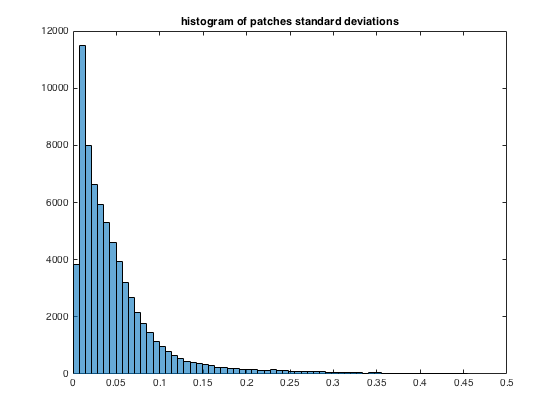
\includegraphics[width=12cm]{images/p1-1-a_std_hist}
				 		\caption{histogram of standard deviations in the xtr dataset after normalisation}
				 		\label{fig:p1-1-a_std_hist}
				 	\end{figure}
				 	The maximum possible value of standard deviation is $\frac{max. - min.}{2}$, so in our case after normalisation it is $\frac{1 - 0}{2}= 0.5$. Our threshold to distinguish discrete values of pixels is $\frac{1}{64} = 0.5 / 32 \approx 0.0156$. If we use 32 bins on a range of possible values of standard deviation (between 0 and 0.5) then the width of one bin will be 0.0156 and standard deviations with values  0.0151 or 0.0021 will go to the same bin. But we usually would associate (after rounding using threshold) standard deviation 0.0151 with the discrete (original) pixel value of 1 and 0.0021 with 0 because $round(0.0151/0.0156)=round(0.968)=1$ and $round(0.0021/0.0156)=round(0.135)=0$. Therefore, we must choose minimum 64 bins in order to distinguish such cases because we will have bins width $\frac{0.5}{64} \approx \frac{0.0156}{2} = 0.0078$ and each bin will correspond to the specific discrete (original) pixel value.\\
				 	From the figure \ref{fig:p1-1-a_std_hist} we can see that after the peak on the second bin (associate it with deviation around 1 discrete pixel value) the number of patches declines exponentially as  standard deviation increases . We can conclude that most of patches have standard deviation within 0 and 0.05 range, and 0.05 is quite small standard deviation, therefore, most of the patches are flat ones. \\
				 	Code snippet to plot histogram:
				 	\lstinputlisting{code/tsk1_1_a.m}
				 	
				\item
					I would chose the mean of all pixels in the patch as simple predictor for flat patches. Given the definition of flat patches $the intensity of the pixel_{i}$in the flat patch should be something like this $f_{i}(\vect{x_{all\ other\ pixels}}) = const_{this flat\ patch} + o(\vect{x_{all\ other\ pixels}})$ where o is small function in comparison to $const_{flat\ patch}$, and its mean and standard deviation over all pixels in the patch are 0 and as $\sigma_{flat\ patch}$ respectively. For flat patches the following is true $\sigma_{flat \, patch} \leq \sigma_{flat \, pach \, max}$. So it is natural to propose  $const_{this flat\ patch}$ as our prediction, which can be received by calculating mean over all pixels in the flat patch\\
					The performance of this simple predictor can be estimated by considering extreme case when after normalisation (all pixel values between 0 and 1) most pixels are zeroes and small portion of pixels are ones (correspond to original intensity of 63). Let $N-m$ be number of zeros and let $m$ be number of ones and I denote $\mu$ as mean. 
					\begin{gather*}
						m < N - m\\
						\mu = \frac{(N - m) * 0 + m * 1}{N} = \frac{m}{N}\\
						\sigma^2 = (N - m) (0 - \frac{m}{N})^2 + m(1 - \frac{m}{N})^2 \\
						= \frac{(N - m)m^2}{N^3} + \frac{m(N - m)^2}{N ^ 3}\\
						N^3\sigma^2 = Nm^2 - m^3 + mN^2 - 2m^2N + m^3 \\
						= mN^2-m^2N\\
						m^2 - mN + N^2\sigma^2 = 0\\
						m = \frac{N}{2}(1 - \sqrt{1 - 4 \sigma ^ 2})\quad\text{(minus because our case is $m < N - m$ )}\\
					\end{gather*}
					putting $\sigma_{flat \, pach \, max} = \frac{4}{63} \approx 0.0635$ instead of $\sigma$ and using $N = 1032$ we get
					\begin{gather*}
						m = \frac{1032}{2}(1 - \sqrt{1 - 4 * 0.0635^2}) \approx 4.178
					\end{gather*}
					rounding m to the closest integer we receive $m = 4$. \\Thus, in most extreme case of flat patch we can have 4 ones (correspond to original pixel intensity of 63) and 1028 zeros, so it is natural that we want to predict zero as discrete value of our target pixel.  The mean gives us $\mu = \frac{1028 * 0 + 1 * 4} {1032} \approx 0.0038$. Dividing range between 0 and 1 by 64 we get 0.0156 as our threshold to distinguish discrete pixel values. $round(0.0038/0.0156)=round(0.244)=0$ so our mean value will correspond to 0 as the discrete value of our target pixel and that is what we wanted.
				\newpage
				\item
				 	\begin{figure}[t]
				 		\centering
				 		\caption{patch images}
				 		\label{fig:patch_images}
						\begin{subfigure}{0.5\textwidth}
											      	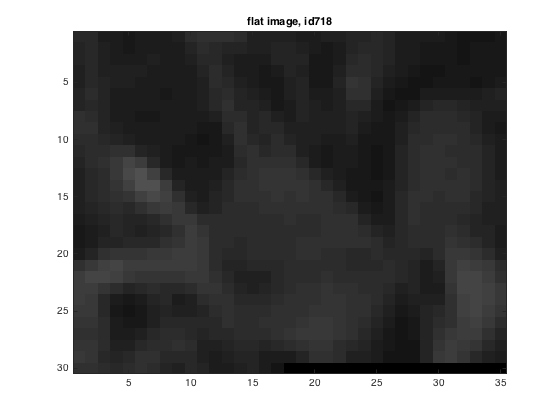
\includegraphics[width=\linewidth]{images/p1-1-c_flat}
											      	\caption{flat patch image}
											      	\label{fig:flat_patch_image}
						\end{subfigure}%
						\begin{subfigure}{0.5\textwidth}
											      	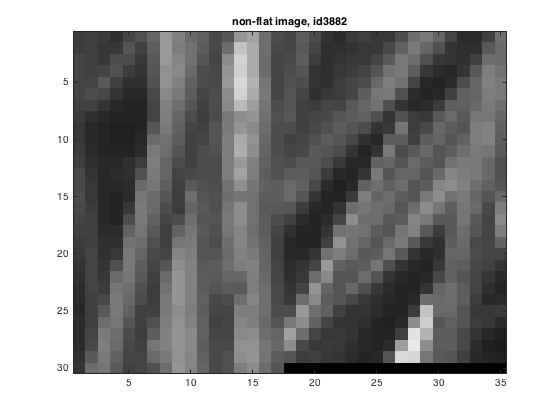
\includegraphics[width=\linewidth]{images/p1-1-c_non_flat}
											      	\caption{non-flat patch image}
											      	\label{fig:non-flat_patch_image}
						\end{subfigure}%
				 	\end{figure}
					 Code snippet to show patch images on figure \ref{fig:patch_images}:
				 	 \lstinputlisting{code/tsk1_1_c.m} 
			\end{enumerate}		
		\subsection{Linear regression with adjacent pixels}
			\begin{enumerate}[label=(\alph*)]
				\item
				 	\begin{figure}[t]
				 		\centering
				 		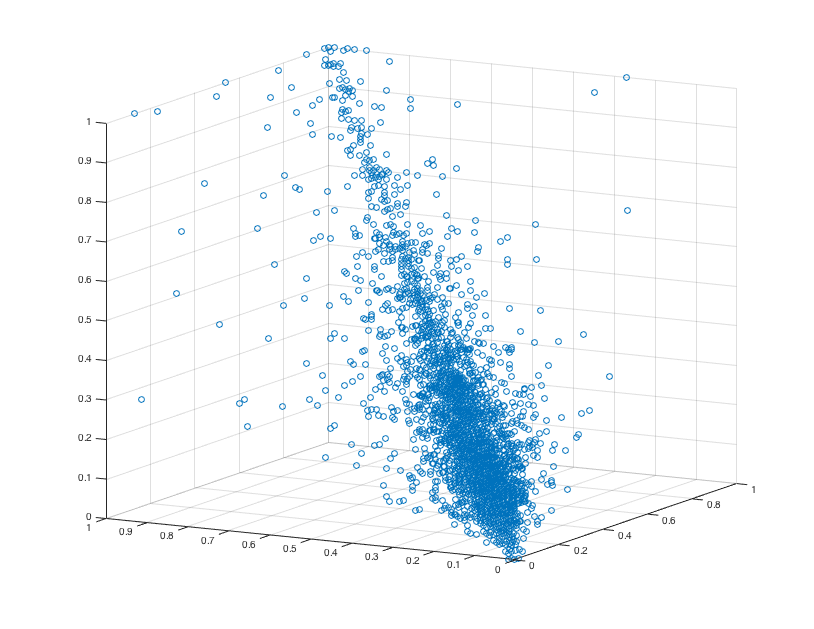
\includegraphics[width=10cm]{images/p1-2-a_closest_pixels}
				 		\caption{scatter plot of adjacent pixels. 5000 data points from xtr\_nf and ytr\_nf}
				 		\label{fig:p1-2-a_closest_pixels}
				 	\end{figure}
					I used 5000 training points from xtr\_nf and ytr\_nf to plot figure \ref{fig:p1-2-a_closest_pixels}. From it we can see that x(j, end), x(j, end - 34), y(j) are strongly positively correlated. However, there is some relatively small number of deviations from this trend. It seems that these deviations are normally distributed so linear regression should be reasonable model to describe such data.\\
					Code snippet for scatter plot:
					\lstinputlisting{code/tsk1_2_a.m} 
				\item
					Derivation of this solution can be taken from MLPR lecture 7 slides 8-11 \href{http://www.inf.ed.ac.uk/teaching/courses/mlpr/2015/slides/07_regression.pdf}{here}. The solution for weights from there is:
					\begin{gather*}
					\hat{\vect{w}} = (\Phi^T \Phi)^{-1} \Phi^T \vect{y}
					\end{gather*}
					In our notation matrix $\Phi$ will become:
					\begin{gather*}
						\Phi = X = 
						\begin{pmatrix}
						1, x(1, end), x(1, end - 34)\\
						1, x(2, end), x(2, end - 34)\\
						\ldots \\
						1, x(N, end), x(N, end -34)
						\end{pmatrix} \\
						\hat{\vect{w}} = (X^T X)^{-1} X^T \vect{y}
					\end{gather*}
					where N is a number of training data points and x is our dataset (it will be xtr\_nf in the next task)
				\item
					code snippet to get linear regression predictor (will be used afterwards):
					\lstinputlisting{code/cs_linear_regression.m} 
					code snippet to compute root mean square error (RMSE) (will be used afterwards):
					\lstinputlisting{code/cs_rmse.m}
					code snippet for this task:
					\lstinputlisting{code/tsk1_2_c.m}
					after training the weights are:
					\begin{center}
						\begin{tabular}{| c | c | c |}
							\hline
							bias & left pixel & above pixel \\ \hline
							0.0026  & 0.4606 & 0.5241 \\ 
							\hline
						\end{tabular}
					\end{center}					
					the RMSE for test and training sets:
					\begin{center}
						\begin{tabular}{| c | c | c |}
							\hline
							\, & Training set & Test set \\ \hline
							RMSE  & 0.0506 & 0.0503 \\ 
							\hline
						\end{tabular}
					\end{center}
				 	\begin{figure}[t]
				 		\centering
				 		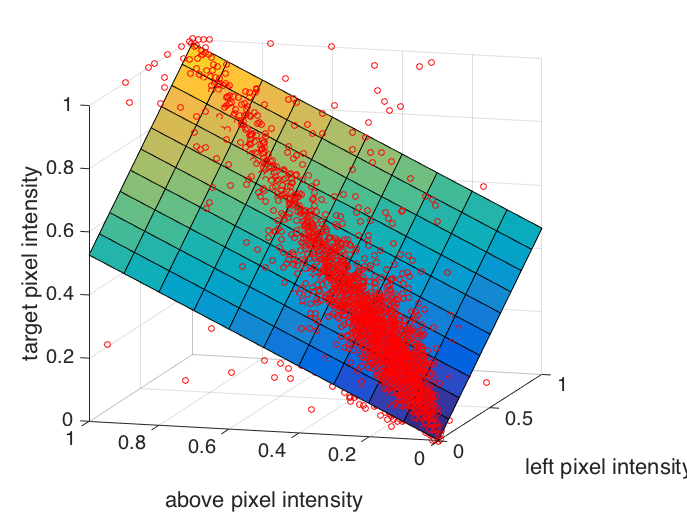
\includegraphics[width=10cm]{images/p1-2-c}
				 		\caption{plot of the linear regression function after training along with test data points}
				 		\label{fig:p1-2-c}
				 	\end{figure}
					This is not a typo, surprisingly my performance is a bit better on the test set. That is why we can conclude that linear regression is not over-fitting the data in this problem. It can be seen from figure \ref{fig:p1-2-c} that indeed there is strong positive correlation between adjacent pixels and target value pixel. 
			\end{enumerate}
			\newpage
		\subsection{RBF regression with adjacent pixels}
			\begin{enumerate}[label=(\alph*)]
				\item
				 	\begin{figure}[t]
				 		\caption{Root Mean Square Error against number of radial basis functions used}
				 		\begin{subfigure}{0.5\textwidth}
				 			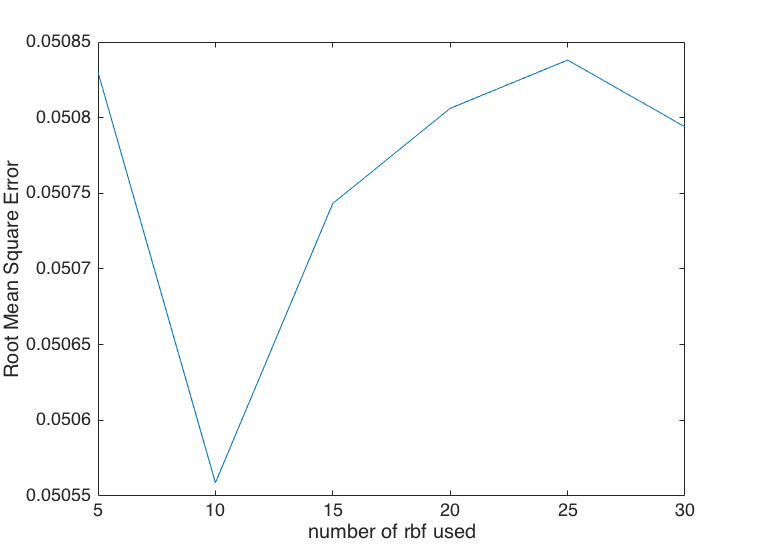
\includegraphics[width=\linewidth]{images/p1-3-a_5_30.png}
				 			\caption{}
				 			\label{fig:p-1-3-a_a}
			 			\end{subfigure}
				 		\begin{subfigure}{0.5\textwidth}
				 			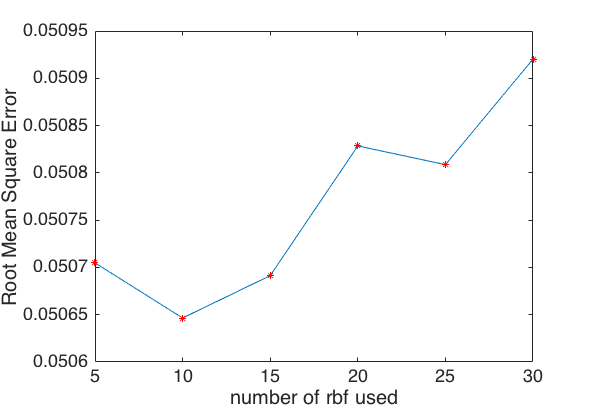
\includegraphics[width=\linewidth]{images/p1-3-a_5_30_another.png}
				 			\caption{}
				 			\label{fig:p-1-3-a_b}
				 		\end{subfigure}\\
				 		\begin{subfigure}{0.5\textwidth}
				 			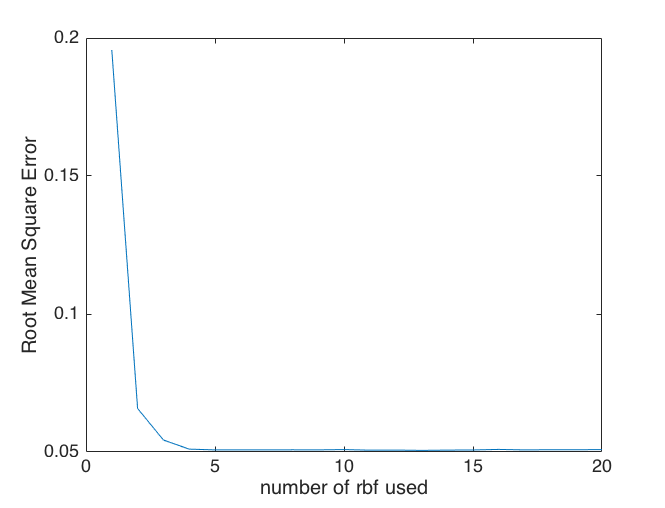
\includegraphics[width=\linewidth]{images/p1-3-a_1_20.png}
				 			\caption{}
				 			\label{fig:p-1-3-a_c}
				 		\end{subfigure}

				 	\end{figure}	
				 	Code snippet for this task:
				 	\lstinputlisting{code/tsk1_3_a.m}
				 	When I ran cross validation procedure to determine which number of radial bases functions among \{ 5, 10, 15, 20, 25, 30\}  produces the best results, each time I received a different answer.  The figure \ref{fig:p-1-3-a_a} suggests 5 as the best number of radial bases functions and \ref{fig:p-1-3-a_b} proposes 10 as the best choice. This happens probably due to the random numbers as matlab crossval uses them each time to divide input set on training and validation sets and rbf network initialises weights differently depending on the random numbers. After that I launched the procedure for number of radial basis functions between 1 and 20, and I have realised that it was just a matter of scale. The figure \ref{fig:p-1-3-a_c} demonstrates that we achieve almost no improvement if we use more than 5 radial bases functions in this task. That is why I have chosen 5 as my number of radial basis functions because for the same efficiency it takes less time to compute.
				 	
				 \item
					the RMSE for test and training sets:
					\begin{center}
						\begin{tabular}{| c | c | c |}
							\hline
							\, & Training set & Test set \\ \hline
							RMSE  & 0.0506 & 0.0503 \\ 
							\hline
						\end{tabular}
					\end{center}
					As it can be seen that radial basis functions don't give any sufficient improvement in comparison to linear regression when both of them are using only adjacent pixels as features.
				 	Code snippet for this task:
				 	\lstinputlisting{code/tsk1_3_a.m}
			\end{enumerate}
			 
		\subsection{Linear regression with all pixels}
			the RMSE for test and training sets:
			\begin{center}
				\begin{tabular}{| c | c | c |}
					\hline
					\, & Training set & Test set \\ \hline
					RMSE  &  0.0371 & 0.0456 \\ 
					\hline
				\end{tabular}
			\end{center}
			There is an improvement comparing with both previous methods but on the test set it is quite small. Overall, it is possible to conclude that whereas knowledge of all the pixels helps to predict the value of target pixel better, indeed, the most significant features are pixels adjacent to the target one.
			Code snippet for this task:
			\lstinputlisting{code/tsk1_4.m}
		\subsection{Neural Network with all pixels}
			\begin{enumerate}[label=(\alph*)]
				\item
					the RMSE for test and training sets:
					\begin{center}
						\begin{tabular}{| c | c | c |}
							\hline
							\, & Training set & Test set \\ \hline
							RMSE  &  0.0333 & 0.0473 \\ 
							\hline
						\end{tabular}
					\end{center}
					In comparison to linear regression with all pixels Neural Network slightly over-fits the data because  its error is lower on training set but the error on test set is larger.\\
					Code snippet for this task:
					\newpage
					\lstinputlisting{code/tsk1_5_a.m}
					
				\item
					Neural Network RMSE for different random seeds:
					\begin{center}
						\begin{tabular}{| c | c | c |}
							\hline
							random seed & RMSE on training set & RMSE on test set\\ \hline
							2015 & 0.0500 & 0.0515 \\ 
							2016 & 0.0477 & 0.0504 \\ 
							2017 & 0.0485 & 0.0515 \\ 
							2018 & 0.0477 & 0.0516 \\ 
							2019 & 0.0489 & 0.0527 \\
							\hline
						\end{tabular}
					\end{center}
					The average values for different random seeds are 0.0486 and 0.0515 for training and test sets respectively. In comparison to previous task 1.5.a the difference between training and test errors is much smaller in all cases because we are not using all the training instances for learning. At the same time, most likely due to the same reason, our performance on the training and test set has dropped. \\
					Random seed determines to what local minimum NN will try to converge. That is why if we have a lower error on the training set then it is not guaranteed that our test error will be lower, as well. Runs with random seeds 2015 and 2019 are examples of this.\\
					Code snippet for this task:
					\lstinputlisting{code/tsk1_5_b.m}
			\end{enumerate}
		\subsection{Discussion}
		 	\begin{figure}[t]
		 		\centering
		 		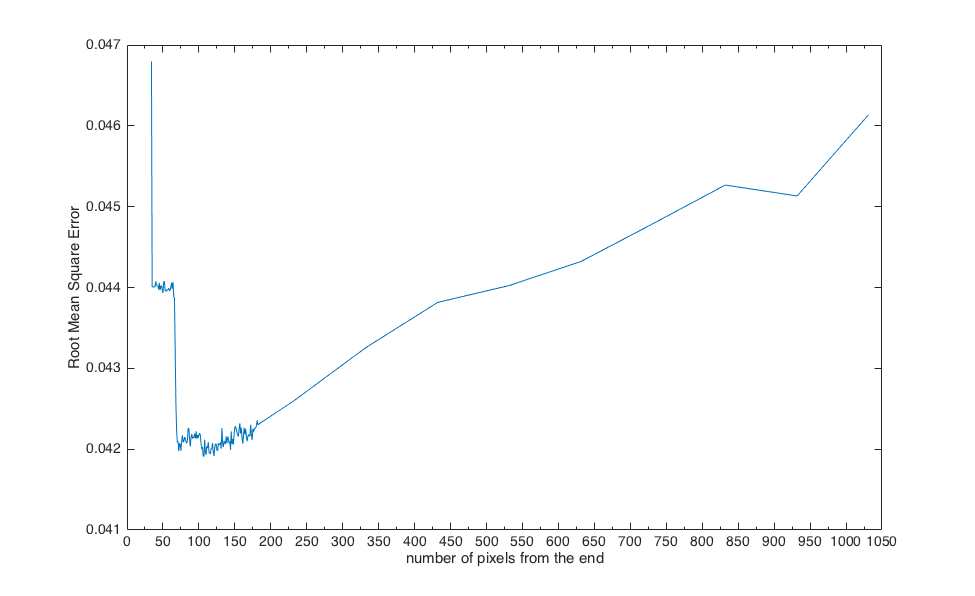
\includegraphics[width=17cm]{images/p1-6_num_pixels.png}
		 		\caption{plot of linear regression RMSE depending on the number of pixels from the end  used as features.}
		 		\label{fig:p1-6_num_pixels}
		 	\end{figure}
		 	\begin{figure}[t]
		 		\centering
		 		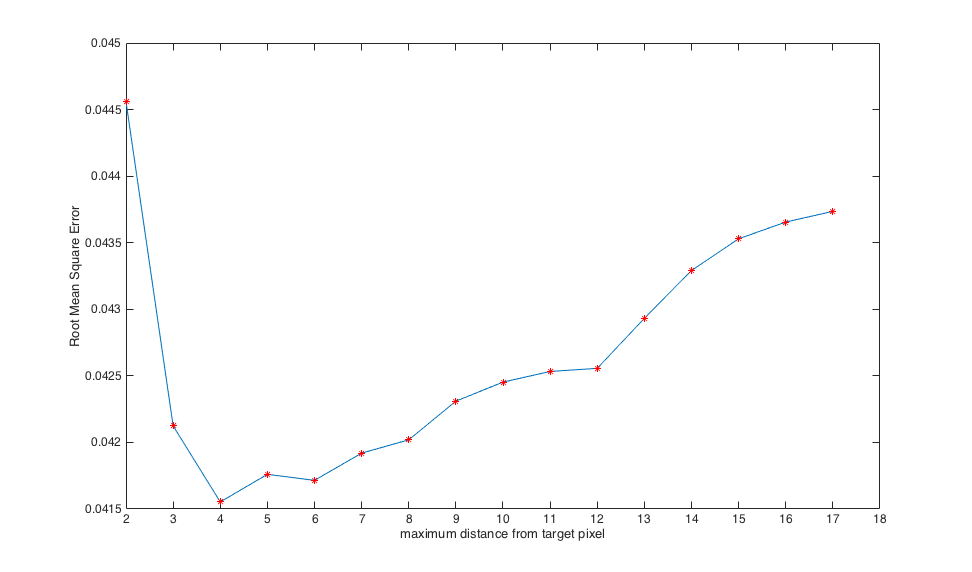
\includegraphics[width=17cm]{images/p1-6_closest_pixels.png}
		 		\caption{plot of linear regression RMSE depending on the maximum distances from the target pixels within which pixels were  used as features.}
		 		\label{fig:p1-6_closest_pixels}	
		 	\end{figure}
		 	In previous tasks linear regression with all pixels showed the best performance. That is why I thought that it would be reasonable to try something else with linear regression. It seemed to me that the adjacent pixels have the biggest impact on the intensity of the target pixel. But how many nearest pixels do we need? I wasn't sure so I evaluated linear regression performance depending on the number of pixels from the end of feature vector via cross-validation on the training set. The result can be seen on the figure \ref{fig:p1-6_num_pixels}. \textbf{Note}: the plot step is not uniform, after 182 I used much bigger step because otherwise cross-validation would take too much time.\\ Figure suggests that the best value is something like 120. Using that number of feature on the test set (xte\_nf(:, 912:1032)) I received the following RMSE:
			\begin{center}
				\begin{tabular}{| c | c | }
					\hline
					\, &  Test set \\ \hline
					RMSE & 0.0419 \\ 
					\hline
				\end{tabular}
			\end{center}
			
			This result shows improvement in comparison to the previous models. Also we can see that at the beginning figure \ref{fig:p1-6_num_pixels} has form similar to the step function. I describe it by the fact that with period of 35 we receive pixels which are above the target one and they give a lot of information about target pixels. This leads to conclusion that if image is 2d-array of pixels where i, j are indexes on the X and Y axis respectively then we should select pixels/features depending on their euclidean distance from the target pixel $r = \sqrt{(18 - i)^2 + (30 - j)^2}$. \\
			Code snippet to get the closest pixels:
			\lstinputlisting{code/get_closest_pixels.m}
			
			 I have performed cross-validation on the training set to find best such distance, the results are on figure \ref{fig:p1-6_closest_pixels}. It points out that the best distance is 4, and after checking it on the test set:
			\begin{center}
				\begin{tabular}{| c | c |}
					\hline
					\, &  Test set \\ \hline
					RMSE & 0.0412 \\ 
					\hline
				\end{tabular}
			\end{center}
			This is the best result among the models considered and this model is computationally efficient because it needs to take only 21 closest pixels in contrast to linear regression or Neural Network with all the pixels. \\ 
			Code snippet to plot figure \ref{fig:p1-6_num_pixels}:
			\lstinputlisting{code/tsk1_6_1.m}
			Code snippet to get performance on the test set using 120 pixels from the end:
			\lstinputlisting{code/tsk1_6_2.m}
			Code snippet to plot figure \ref{fig:p1-6_closest_pixels}:
			\lstinputlisting{code/tsk1_6_3.m}
			Code snippet to get performance on the test set with pixels within radius 4 from target one:
			\lstinputlisting{code/tsk1_6_4.m}
			\newpage
			
		\section{Robust modelling}
			\section*{Note}
				It is assumed that I have loaded the code from \href{http://www.inf.ed.ac.uk/teaching/courses/mlpr/2015/assignment/part2_code_data.tar.gz}{part2\_code\_data.tar.gz} in my matlab environment. I have also taken professor Iain Murray code from MLPR tutorial 5 to produce error bars - \href{http://homepages.inf.ed.ac.uk/imurray2/code/imurray-matlab/errorbar_str.m}{errobar\_str.m}. text\_data.mat is assumed to be loaded as well.
			\subsection{Fitting the baseline model}
				\begin{enumerate}[label=(\alph*)]
					\item 
						The code snippet to add bias term:
						\lstinputlisting{code/tsk2_1_a.m}
					\item
						I have received the following results:
						\begin{center}
							\begin{tabular}{| c | c | c |}
								\hline
								\, &  Test set \\ \hline
								RMSE & 0.0412 \\ 
								\hline
							\end{tabular}
						\end{center}
				\end{enumerate}
				
				
\end{document}
